To attempt at reconstructing the latent signal from incomplete observations, it is generally of interest to understand the underlying statistics, as this informs both noise characteristics and the likelihood of different observations. In many imaging and detection systems, especially those involving photons and photoelectron emissions, the observed data is inherently stochastic. Classical and quantum optics provide a comprehensive theoretical foundation to explain photon statistics. For instance, it is well understood that photons from a coherent light source follow a Poisson distribution (an outcome \cref{sec:poisson-noise-model} was based on), often referred to as shot-noise. Whereas, for chaotic (bunched) light, the variance exceeds that compared to their mean, dubbed super-Poissonian. And finally for a squeezed light source, the distribution is sub-Poissonian \cite[Chapter~5]{foxQuantumOpticsIntroduction2006}. The same principle can be extended to photoelectron emission. When photons interact with a material, the resulting photoelectron emission follows the same statistical behavior as the incident photons \cite{mandelFluctuationsPhotonBeams1958,mandelFluctuationsPhotonBeams1959}. 

In this chapter, we begin by formally defining a general model for describing photoelectron event data using a \gls{PPP}, that captures the Poisson-distributed counting statistics for coherent light sources and the \gls{NB} distribution for \gls{SASE} \glspl{FEL}. These model are then tested for counting statistics of photoemitted electrons on data from a pulsed coherent light source and a \gls{SASE} \gls{FEL}.

\section{Modelling Photoelectron Statistics}\label{section:photoelectron-counting-stats}
Let us start by developing an intuition for why photons exhibit stochastic behavior. Photons are the quantized form of electromagnetic light and can be thought of as discrete energy packets. The energy of a photon is given by $E = h\nu$, where $h$ is the Planck constant and $\nu$ is the frequency of the light. Due to the discrete nature of photons, it can be shown that the number of photons in a short time interval $\Delta t$ is not constant. These fluctuations are known as photon shot noise.

For a light source with a constant flux\footnote{Flux is the average number of photons passing through the cross-section of a beam per unit time.} $\phi$ such as a single-mode laser, the average number of photons in a beam segment of length is given by $L$, $\lambda = \phi \frac{L}{c}$, where $c$ is the speed of light. If we subdivide this $L$ into many small intervals  of size $L/N$, where $N$ is large enough so that there is low probability of a photon being in an interval, eventually there will be divisions with no photons, divisions with only single photon, and negligible divisions with multiple photons. For all possible orderings, the probability of finding $n$ subdivisions with a single photon and $(N-n)$ with no photons can be modeled by the Binomial distribution as follows, with $p=\frac{\lambda}{N}$ being the probability of a photon being in a segment:

\begin{equation}
    P(n) = \binom{N}{n} p^n (1 - p)^{N - n}
\end{equation}

Using the Poisson Limit Theorem \cite{fellerIntroductionProbabilityTheory1991a}, it can be shown that as $N \to \infty$, and the probability $p \to 0$ such that $Np = \lambda$ remains constant, there is a convergence in distribution to the Poisson distribution (\cref{note:poisson-distribution}). Hence, the Poisson distribution is a suitable model for counting statistics of photons from a coherent light source.

\subsection{Photoelectron Counting}
\citeauthor{mandelFluctuationsPhotonBeams1958} \cite{mandelFluctuationsPhotonBeams1958,mandelFluctuationsPhotonBeams1959} and others have shown that the transition probability of an electron from its ground state to an unbounded state at the surface of a photodetector is directly proportional to both the duration of the time interval $\Delta t$ and the instantaneous light intensity $I(t)$. This suggests that the rate density of photoelectrons is proportional to the light intensity $\lambda(t) \propto \int_{A} I(t)$, where $A$ is the detector area.

The aforementioned can be mathematically formalized through one-dimensional stochastic process known as a \gls{PP}\footnote{For a more generalized description of \gls{PP}, the reader is referred to \cite{chiuStochasticGeometryIts2013}.}. A \gls{PP} is used to model occurrences of stochastic events that happen in some space. If we look at the time domain, the \gls{PP} allows us to the model the occurrence of events in time. The process generates a series of time points $\{t_1, t_2, \dots, t_n\}$ where the events occur, within a time interval $[0, T]$.

A \gls{PP} often used to model events is the \glsxtrfull{PPP}, describable by the rate density function $\Lambda(t)$ (also known as the intensity function). The key property of such a process is that the events are statistically independent:

\begin{equation}
    \Lambda(t_1, t_2, \dots, t_n) = \prod_{i=1}^{n} \Lambda(t_i)
\end{equation}

If the rate density function is constant, $\Lambda(t) = \Lambda$, the process is known as a homogeneous (or stationary) \gls{PPP}, such as the case with a coherent laser light source \cite{salehPhotoelectronStatistics1978}. If the rate function is time-dependent and deterministic $\Lambda(t)$, it is known as the inhomogeneous \gls{PPP}. Such a situation could occur when the intensity of light is modulated, as is the case with a pulsed laser source. In a situation such as where the $\Lambda(t)$ itself is a stochastic variable, the process is known as the doubly stochastic \gls{PPP}, or Cox process. 

% Such is the case if the light source is a \gls{SASE} \gls{FEL}, where the intensity of light fluctuates stochastically (see \cref{section:light-sources} for why this happens). Due to this process, the photoelectron counting statistics in this case also deviate from the Poisson distribution, as we shall see later.

Integrating light intensity $I(t)$ over the time interval $\Delta t$ can be treated as a random variable with probability density $P(W)$, with $W$ as:
\begin{equation}
    W = \int_{\Delta t}^{t+\Delta t} I(t') dt
\end{equation}

The probability of detecting $n$ photoelectrons in that time interval is then given by the Poisson transform relation \cite{mehtaVIIITheoryPhotoelectron1970} (a realization of the doubly stochastic \gls{PPP}):
\begin{equation}\label{eq:mandel-photo-electron}
    P(n, t, \Delta t) = \int_{0}^{\infty} \frac{\alpha W^n}{n!} e^{-\alpha W} P(W) \, dW
\end{equation}

With a constant intensity light source, $W$ becomes deterministic and \cref{eq:mandel-photo-electron} simplifies to a Poisson distribution:
\begin{equation}
    P(n, t, \Delta t) = \frac{W^n e^{-W}}{n!} 
\end{equation}

Due to the \gls{SASE} process of an \gls{FEL} light, discussed briefly in \cref{section:light-sources}, the light intensity fluctuates stochastically. This leads to the photoelectron counting statistics being over dispersed and deviating from the Poisson distribution. \citeauthor{saldinStatisticalPropertiesRadiation1998} have shown in \cite{saldinStatisticalPropertiesRadiation1998} that the photoelectron counting statistics from a \gls{SASE} \gls{FEL} light source can be modeled by a \gls{NB} distribution (\gls{PMF} and other details defined in \cref{note:negative-binomial-distribution}), a realization of the Cox process. And due to the light and photoelectron statistics relation, the photoelectron counting statistics also follow the same distribution.

The important thing to note here is that above discussion is about the statistics of photoelectrons from photon detection. Whereas, our experiment is of \gls{PES}, where we are then interested in the (detected) emitted electrons (electron count distributions).

\section{Testing of Counting Statistics}
There are two simple ways to test a \gls{PPP}\footnote{Specialized statistical tests do exist to directly test for a homogeneous \gls{PP}, hypothesizing complete spatial randomness. Ripley's K-function can be used as a goodness of fit test \cite[Section~2.6.4]{chiuStochasticGeometryIts2013}. However, these do not test for the doubly stochastic \gls{PPP}.}. \textit{The interval statistics}, where the time intervals between events $\Delta t$ should follow an exponential distribution for a \gls{PPP}. The other is \textit{counting statistics}, where the number of events ($\gls{ncounts}$) within a fixed time interval $\Delta t$ should follow a distribution based on \cref{{eq:mandel-photo-electron}}.

We consider the latter case, for two reasons. First, from the discussion above, we have well-established hypotheses between the expected distributions for different light sources. Second, the timing information from the light source is coarser than the electron detection time. While the \gls{DLD} detector measures the \gls{TOF} of each electron, allowing us to get individual timing, the detector's dead-time could influence the time-interval statistics. Therefore, we analyze the \textit{counting statistics}.

\begin{figure}
    \centering
    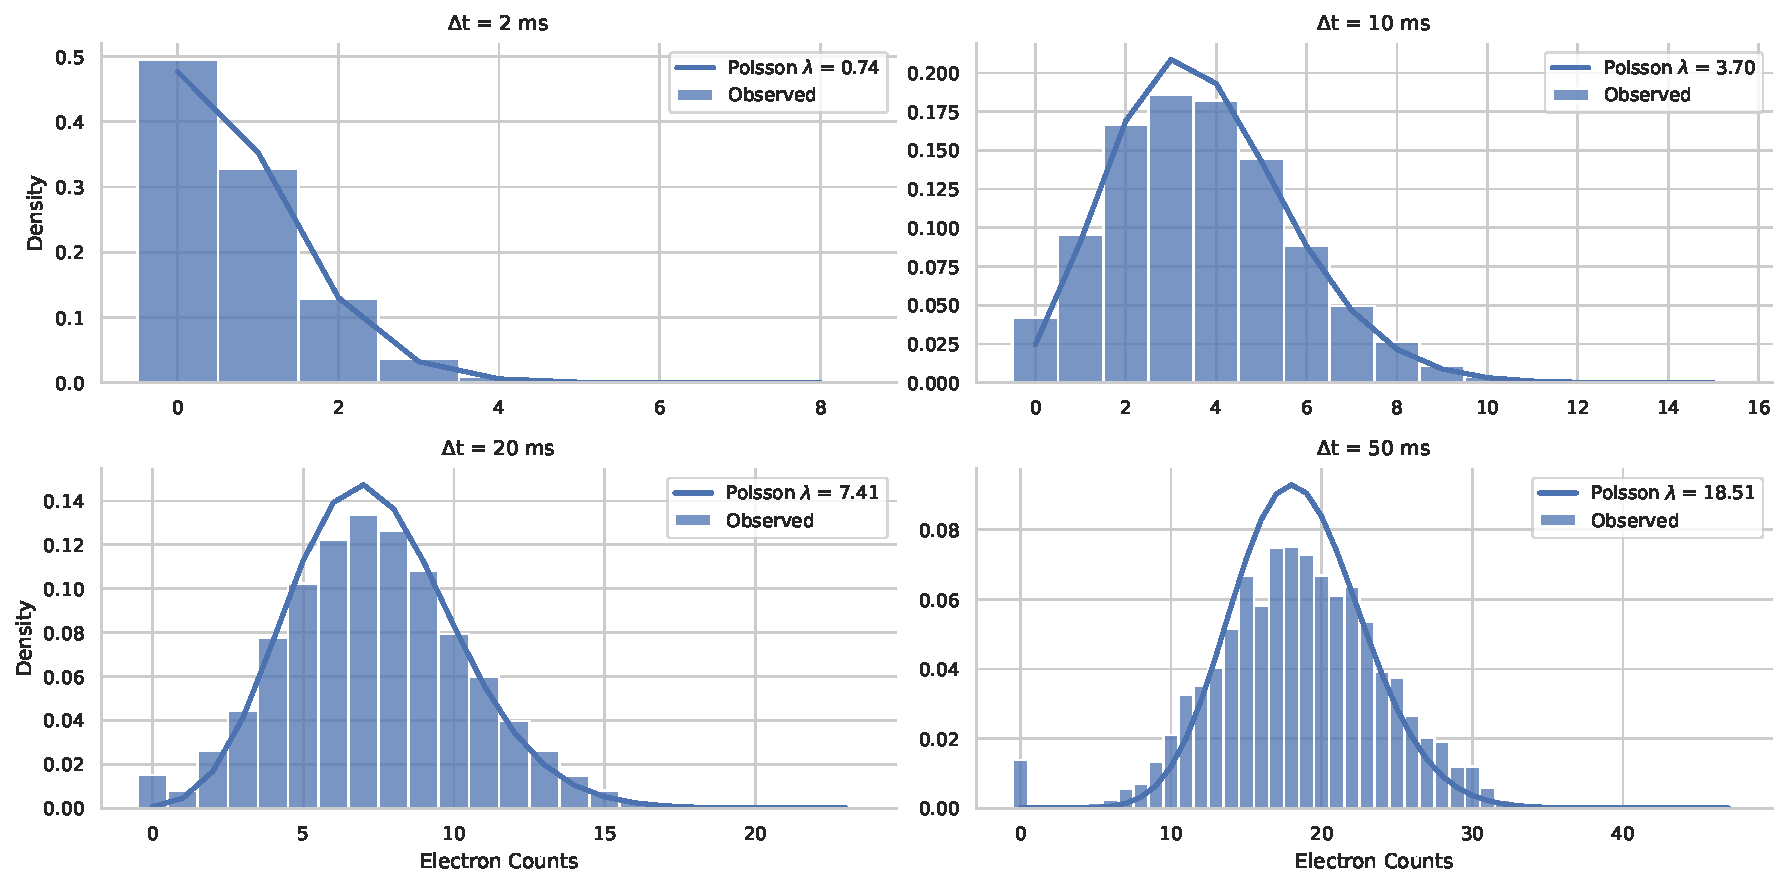
\includegraphics[width=1\linewidth]{images/hist_counts_facetgrid_1_wse2.pdf}
    \caption{Distribution of photoelectron counts at time intervals $\Delta t =$ \qtylist{2;10;20;50}{ms} for a selected volumetric subset of the full \gls{WSe2} dataset. Poisson statistics are observed at smaller time intervals, but as the time window increases ($\Delta t = \qty{50}{ms}$), the data starts to deviate from the Poisson distribution, as spatial correlations become apparent. The total counts in this selected region are $\gls{ncounts}=\num{4.7e4}$ with total observation time $T=\qty{126}{s}$.}
    \label{fig:wse2-stats}
\end{figure}

We test the counting statistics observed for \gls{PES} at two different light sources: a pulsed \gls{HHG} laser (\gls{WSe2} dataset), and a \gls{SASE} \gls{FEL} light source (\gls{GrIr} dataset). Based on theoretical considerations, we hypothesize that the counting statistics of the photoelectrons from the laser source would align a Poisson distribution, and from the \gls{SASE} \gls{FEL} source, with a \gls{NB} distribution. 
% The hypothesized counting statistics are tested using the Poisson dispersion test, and if that is rejected, using the Chi-Square test (for details regarding this, refer to \cref{section:chi-test}).

While the \gls{PPP} should exhibit the same counting statistics for any time window $\Delta t$, practical challenges such as the long-term measurement drifts in intensity, can make that hard to realize. To account for this, we will analyze several time intervals to determine if the statistics remain valid based on the light source used. Given that the goal of \gls{MPES} is to map band structures whose feature sizes are generally much larger than a single voxel, the data inherently exhibits spatial correlations\footnote{Spatial here means in the image space, which also includes the time delay axis.}. An ideal experimental setup to measure counting statistics would instead minimize spatial correlations and allow for long acquisition times to obtain reliable statistical estimates across different time windows.

In our analysis, we consider the detector-defined 3D subsets of data, which are often sparsely populated. While the most precise assessment of counting statistics would involve analyzing a single voxel, the sparsity of the data necessitates examining small subsets of the 3D volume instead. We select sufficiently small $\Delta t$ to ensure that spatial correlations have minimal impact on the observed statistics, and also look at the cases where it is high.

\subsection{HHG Light Source}
Let us look at the dataset using \gls{HHG} laser first: \gls{WSe2}. \cref{fig:wse2-stats} shows the count distribution at $\Delta t =$ \qtylist{2;10;20;50}{ms}, with an observation time $T=\qty{126}{s}$, and one specific volumetric subset. The count distributions for smaller time intervals ($\Delta t = \qtylist{2;10;20}{ms}$) follow Poisson statistics, as expected from an uncorrelated photoemission process where spatial and temporal fluctuations are minimal. However, for longer time intervals ($\Delta t = \qty{50}{ms}$), the distribution starts to deviate from the Poisson distribution. This deviation suggests that spatial correlations, due to the material properties of the sample, become significant enough to impact the distribution. While the impact of pulse light source should be minimal since the time intervals we look at are much longer than the pulse durations, the intensity drifts could also cause the deviation. \cref{fig:wse2-stats-2} shows count statistics from a different volumetric subset, forming the same conclusions.

From the above, we can conclude that the photoemitted electrons statistics are a realization of a \gls{PPP}. \citeauthor{heimerlMultiphotonElectronEmission2024} \cite{heimerlMultiphotonElectronEmission2024} have also recently showed that the emitted electrons show a Poisson distribution with a (coherent) pulsed laser light source.

To determine the homogeneity of the process, if we look at $\Delta t = \qty{50}{ms}$ in both \cref{fig:wse2-stats} and \cref{fig:wse2-stats-2}, the zero counts start forming a bimodal characteristic. This could be attributed to the pulse structure of the laser light source, where the absence of photons between pulses leads to a high occurrence of zero counts. Hence, due to this inhomogeneity in intensity, the  statistics might be better modeled with an inhomogeneous \gls{PPP}. For a pulsed light source with pulse interval $\tau_{\text{pulse}}$, the counting statistics should still be Poisson for $\Delta t >> \tau_{\text{pulse}}$, and otherwise due to regular spacing when no events occur, it is better modeled by an inhomogeneous \gls{PPP}.

% Applying the Poisson dispersion test at a significance level of $\alpha=0.05$ for \num{1000} samples at each $\Delta t$ of \qtylist{2;10;20;50}{ms}, we report $p$-values of \numlist{0.88;0.87;0.10;0.00}, respectively. The test fails to reject the null hypothesis of Poisson distribution for $\Delta t = \qtylist{2;10;20}{ms}$, but rejects it for $\Delta t = \qty{50}{ms}$.

It must be noted that for \gls{HHG} sources, \citeauthor{gorlachQuantumopticalNatureHigh2020} \cite{gorlachQuantumopticalNatureHigh2020} have shown that the highly non-linear \gls{HHG} process can significantly affect the photon statistics. They have shown that depending on the generated harmonic, the photon statistics vary, with some harmonics able to exhibit squeezed light properties, and others over-dispersion. The seventh harmonic (\qty{21.7}{eV}) up-converted to \gls{XUV} via \gls{HHG} was used for the \gls{PES} of \gls{WSe2} \cite{maklarQuantitativeComparisonTimeflight2020}. Hence, in view of the above-mentioned work, further studies are required to understand the photon and the corresponding photoemitted statistics.

\begin{figure}
    \centering
    \begin{subfigure}[t]{0.49\linewidth}
        \centering
        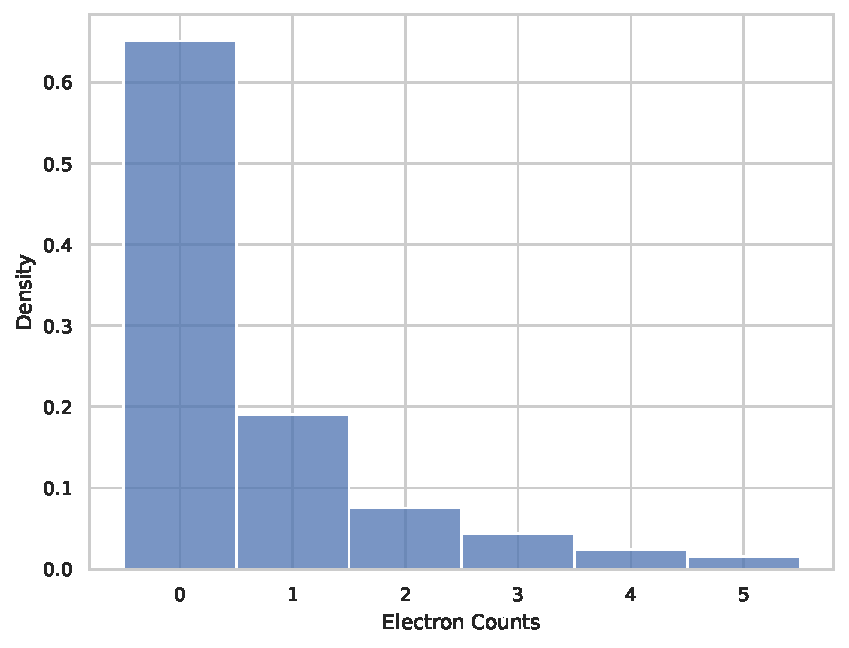
\includegraphics[width=\linewidth]{images/hist_counts_1_layer.pdf}
        \caption{Single layer of the \gls{DLD}.}
        \label{fig:grir-stats-1-layer}
    \end{subfigure}
    \hfill
    \begin{subfigure}[t]{0.49\linewidth}
        \centering
        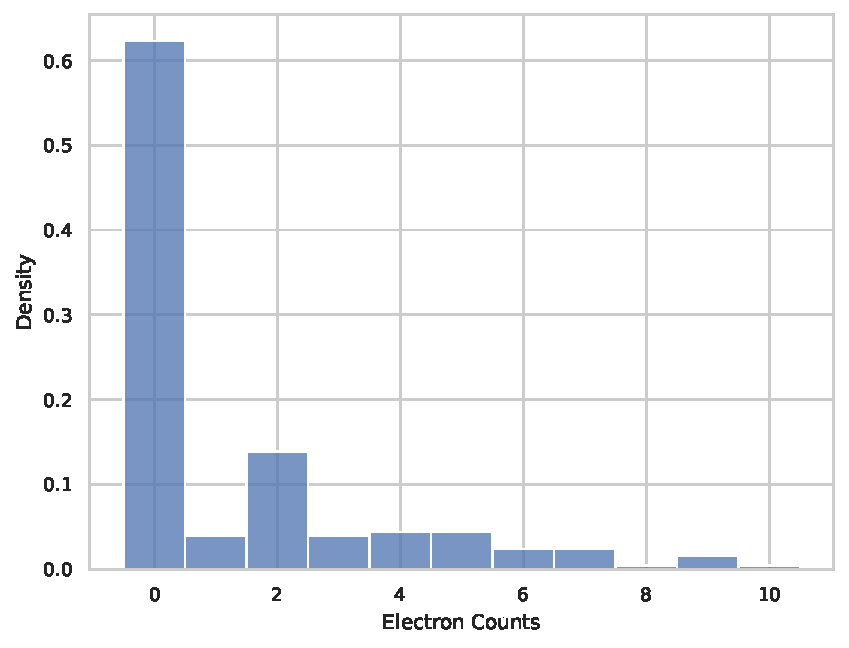
\includegraphics[width=\linewidth]{images/hist_counts_2_layer.pdf}
        \caption{Both layers of the \gls{DLD}.}
        \label{fig:grir-stats-2-layer}
    \end{subfigure}
    \caption{Counting statistics comparison for single layer or both layers of the \gls{DLD}. It is clear that the incorrect counting influences the statistics significantally.}
    \label{fig:grir-stats-dld-comparison}
\end{figure}

\subsection{SASE FEL Light Source}
Analyzing this data requires a few additional considerations. In \cref{section:dld}, we already saw that the \num{8}S \gls{DLD} shows repeated counts for a single electron, due to the segmented structure. From preliminary analysis of counting statistics shown in \cref{fig:grir-stats-dld-comparison}, it can be seen that this has a significant impact on the counting statistics, where the \num{2}-event occurrence is unnaturally high compared to the others (\cref{fig:grir-stats-2-layer}). Therefore, this analysis will only consider a single layer (from the 2-layered delay-line structure), and ideally a volumetric subset from a single segment\footnote{Due to the overlap between segments.}.



\begin{figure}
    \centering
    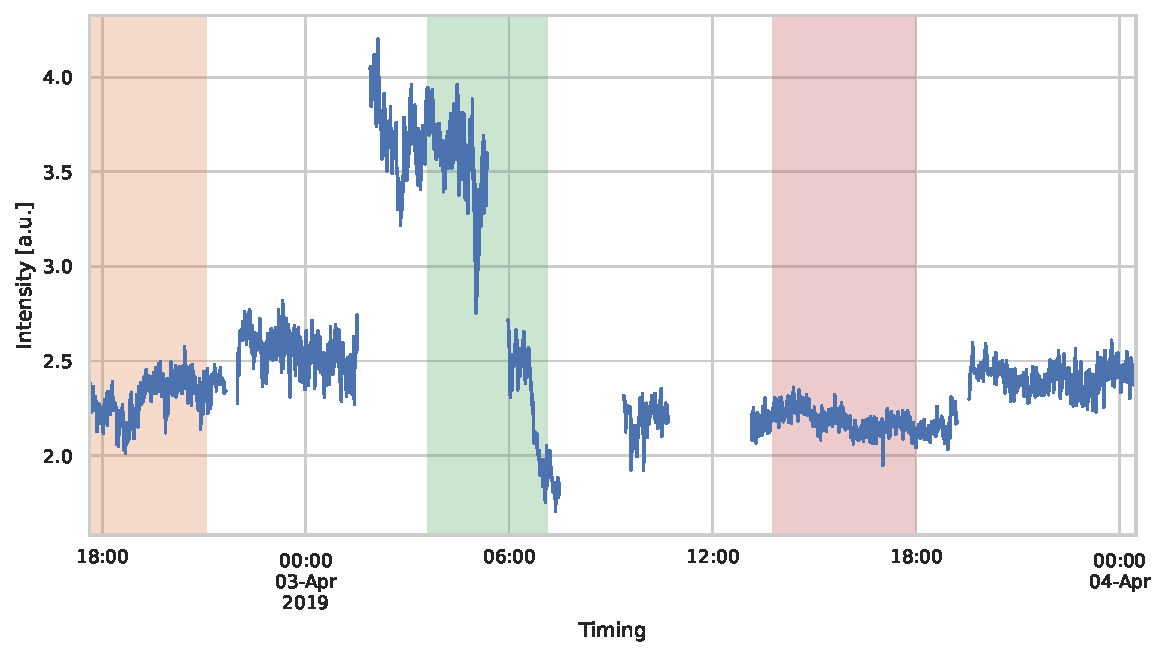
\includegraphics[width=0.8\linewidth]{images/gmd_grir.pdf}
    \caption{Beam intensity measurements, using the \gls{GMD} over the time period $T=\qty{30}{hour}$, with data window-averaged at \qty{1}{min} intervals. The fluctuations in intensity can be observed, an intrinsic property of the \gls{SASE} process. Other notable observations are the long-term drifts in intensity, and the beam interruptions (no recorded values). The orange, green and red spans indicate the time periods used for other analyses.}
    \label{fig:gmd-intensity}
\end{figure}


\begin{figure}
    \centering
    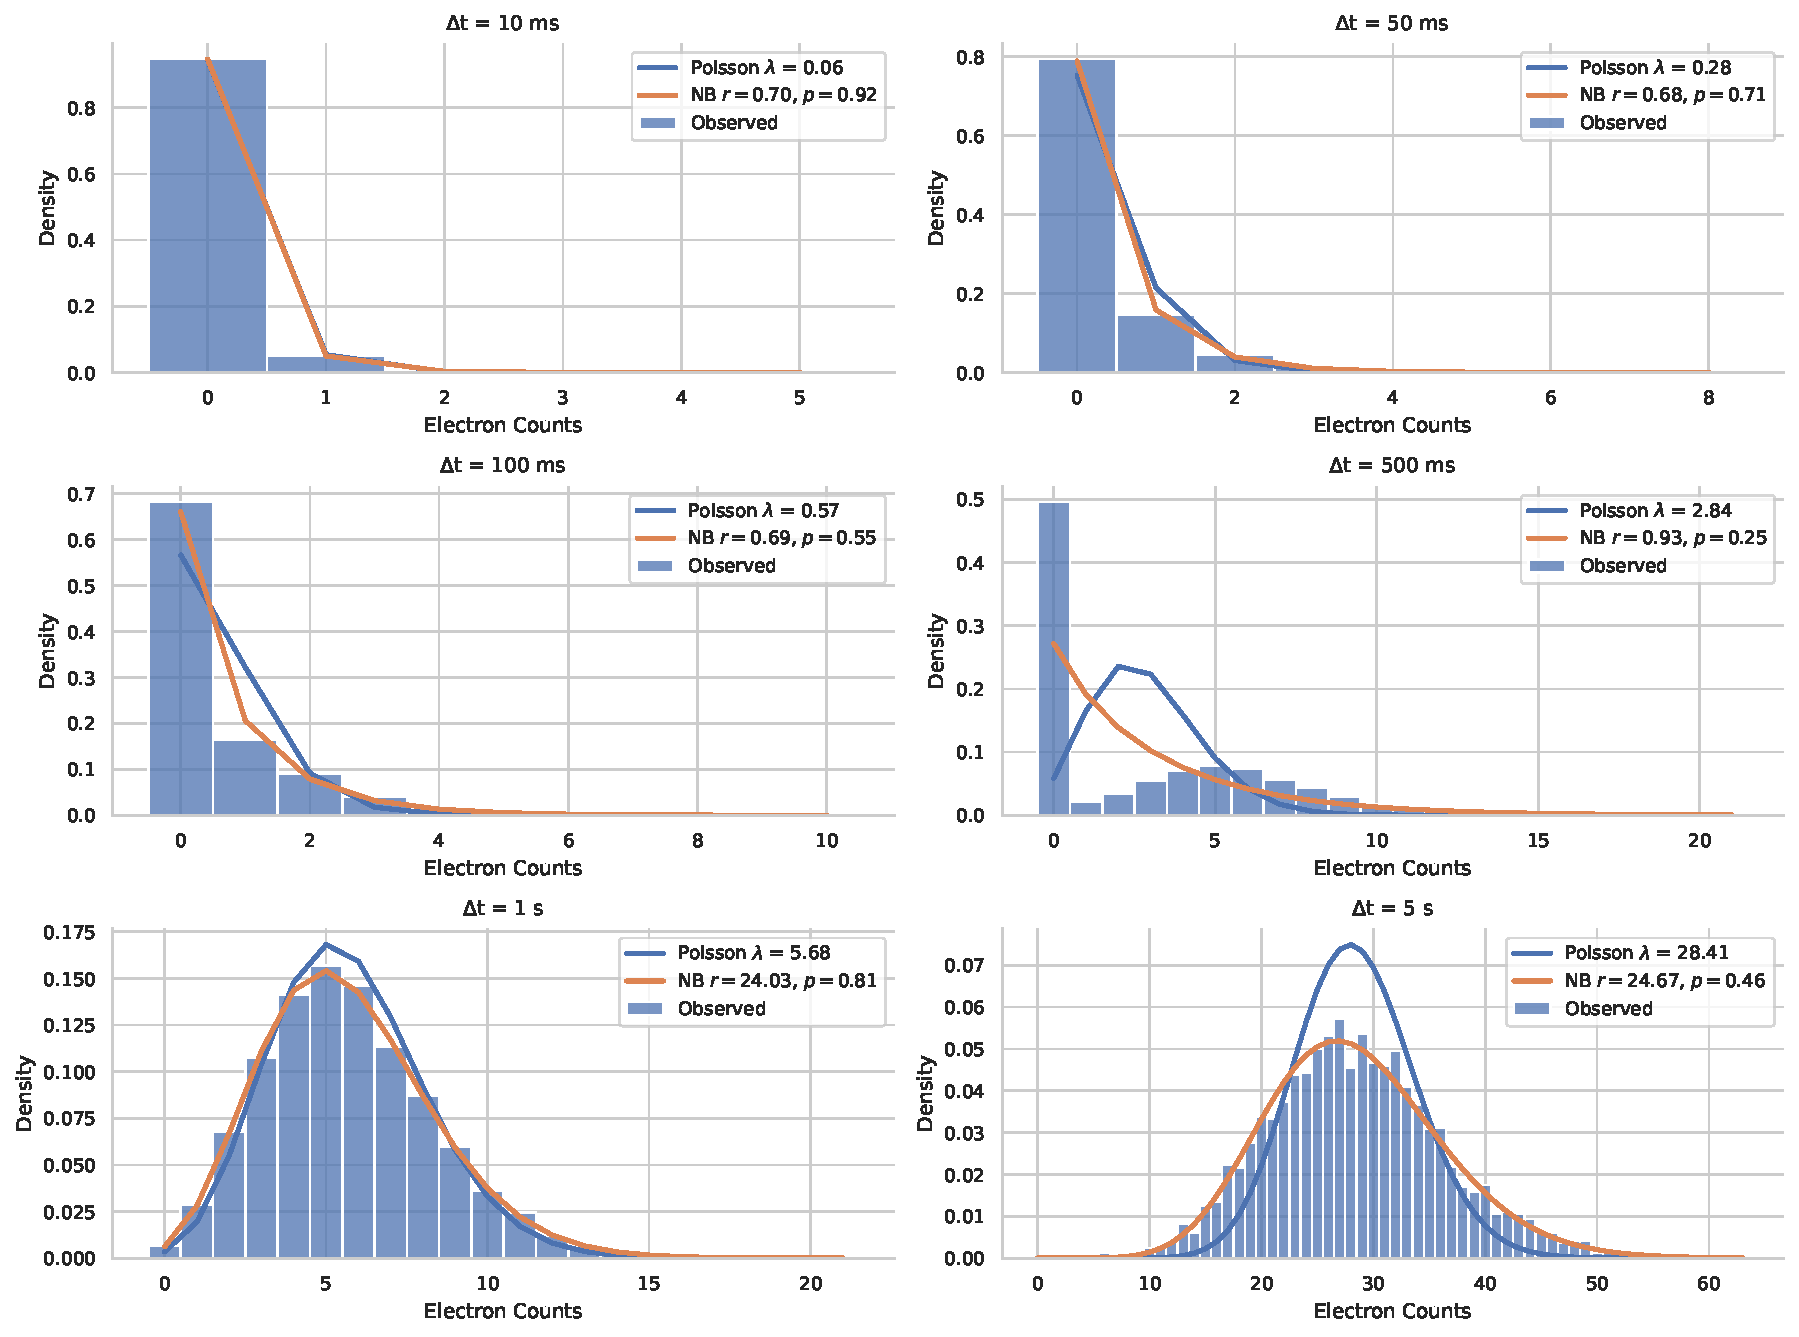
\includegraphics[width=1\linewidth]{images/hist_counts_facetgrid_1_grir.pdf}
    \caption{Distribution of photoelectron counts at time intervals $\Delta t =$ \qtylist{10;50;100;500;1000;5000}{ms} for a selected volumetric subset of the full \gls{GrIr} dataset. At shorter time intervals $\Delta t \leq \qty{50}{ms}$, Poisson statistics provide a good fit, reflecting the limiting case where the \gls{NB} distribution approximates Poisson behavior. However, as the time interval increases, the distribution shows significant over-dispersion, with a pronounced right-skew characteristic of the \gls{NB} distribution. Notably, at $\Delta t = \qty{500}{ms}$, the pulsed structure of the \gls{FEL} becomes apparent, resulting in a high occurrence of zero counts. The total counts for this selected region are \gls{ncounts} = \num{8e5}, with a total observation time of approximately $T = \qty{4}{h}$ (refer to the orange region in \cref{fig:gmd-intensity})}.
    \label{fig:grir-stats-1}
\end{figure}


The second consideration is the long-term intensity drifts in the \gls{FEL} light source. \cref{fig:gmd-intensity} shows the beam intensity measurements\footnote{Measured using \gls{GMD}, see \gls{gmd}} over the time period $T=\qty{30}{hour}$, with data window-averaged at \qty{1}{min} intervals. The long-term drifts in intensity, and the beam interruptions due to accelerator operation can be observed. For analysis, we look at the data from the orange, green, and red spans. With no beam interruptions in the orange and red span, the expectation is that it follows the \gls{NB} distribution. Whereas, the counting statistics would differ in the green span due to the beam interruptions.


We continue looking at the \gls{GrIr} dataset from previous chapters. We look at a broad range of time intervals, as the count rate is much lower compared to the \gls{HHG} source. The pulse structure of the \gls{FEL} is more complex, as illustrated in \cref{fig:hex-tof}. The macrobunches (see \gls{train}) arrive at a repetition rate of \qty{10}{Hz}, meaning a new train of \glspl{pulse} arrives every \qty{100}{ms}.


\cref{fig:grir-stats-1} show photoelectron count distributions for varying time windows ($\Delta t =$ \qtylist{10;50;100;500;1000;5000}{ms}) within the orange span of \cref{fig:gmd-intensity}, with a total observation time of $T=\qty{4}{h}$. At $\Delta t = \qty{10}{ms}$, the Poisson and \gls{NB} fit approximately match. Increasing the time interval starts to show better fit with \gls{NB} than Poisson, with a pronounced right-skew characteristic. Notably, $\Delta t = \qty{500}{ms}$ has a high occurrence of zero counts, which could highlight the pulsed structure of the \gls{FEL}, having regions within each train that have no photons. At $\Delta t = \qty{5000}{ms}$, the deviation from Poisson is apparent, with a significant over-dispersion. \cref{fig:grir-stats-3} shows the same analysis for the red span, with similar conclusions.

\cref{fig:grir-stats-2} shows the interesting regime (green span). The frequency of zero counts clearly deviates from any hypothesis, and is only explainable by the beam interruption, and significant intensity difference. The intensity variation effect is clearly visible at $\Delta t = \qty{5000}{ms}$, where asides from the zero counts, the distribution is bimodal, highlight two distinct count rates.

In summary, the analysis of photoelectron counting statistics from the \gls{FEL} light source highlights the complexity of the data influenced by the detector’s structure, the \gls{SASE} and long-term intensity fluctuations. The \gls{NB} distribution is shown to be a more suitable model for such case. However, for the aim of reconstructing the latent distribution from incomplete observations, the spatial correlations induced by the material under study, and the detector structure should also be considered in the estimation process.


\begin{figure}
    \centering
    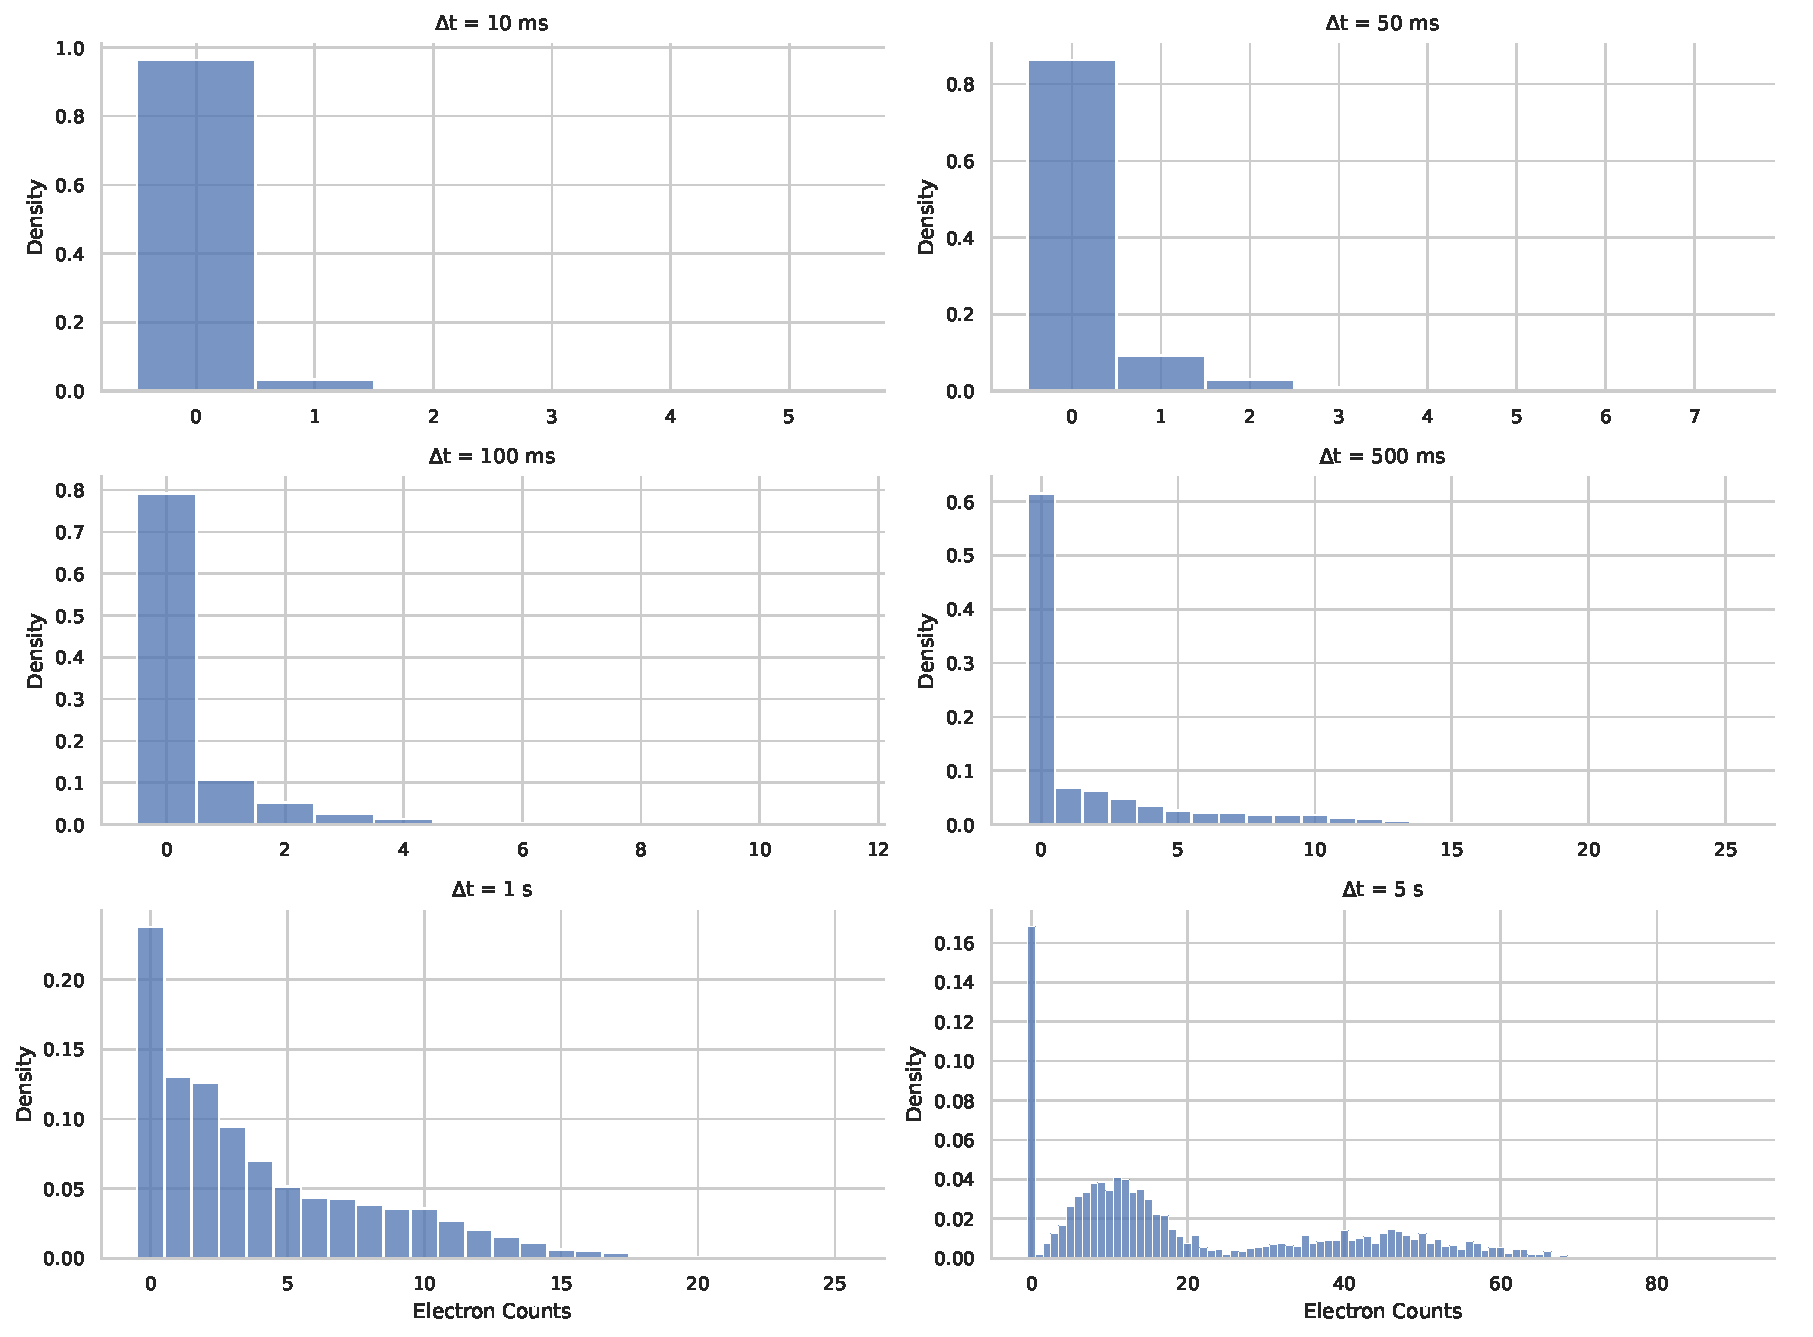
\includegraphics[width=1\linewidth]{images/hist_counts_facetgrid_2_grir.pdf}
    \caption{Distribution of photoelectron counts at time intervals $\Delta t =$ \qtylist{10;50;100;500;1000;5000}{ms} for a selected volumetric subset of the full \gls{GrIr} dataset. The total counts in this selected region are $\gls{ncounts}=\num{5e5}$ with total observation time $T\approx\qty{3.5}{h}$  (See green region in \cref{fig:gmd-intensity}). Neither Poisson nor \gls{NB} statistics provide a good fit for any of the time intervals. The frequency of zero counts is significantly higher, and the distribution is bimodal at $\Delta t = \qty{5000}{ms}$, indicating a significant intensity difference.}
    \label{fig:grir-stats-2}
\end{figure}

% \begin{figure}[t]
%     \centering
%     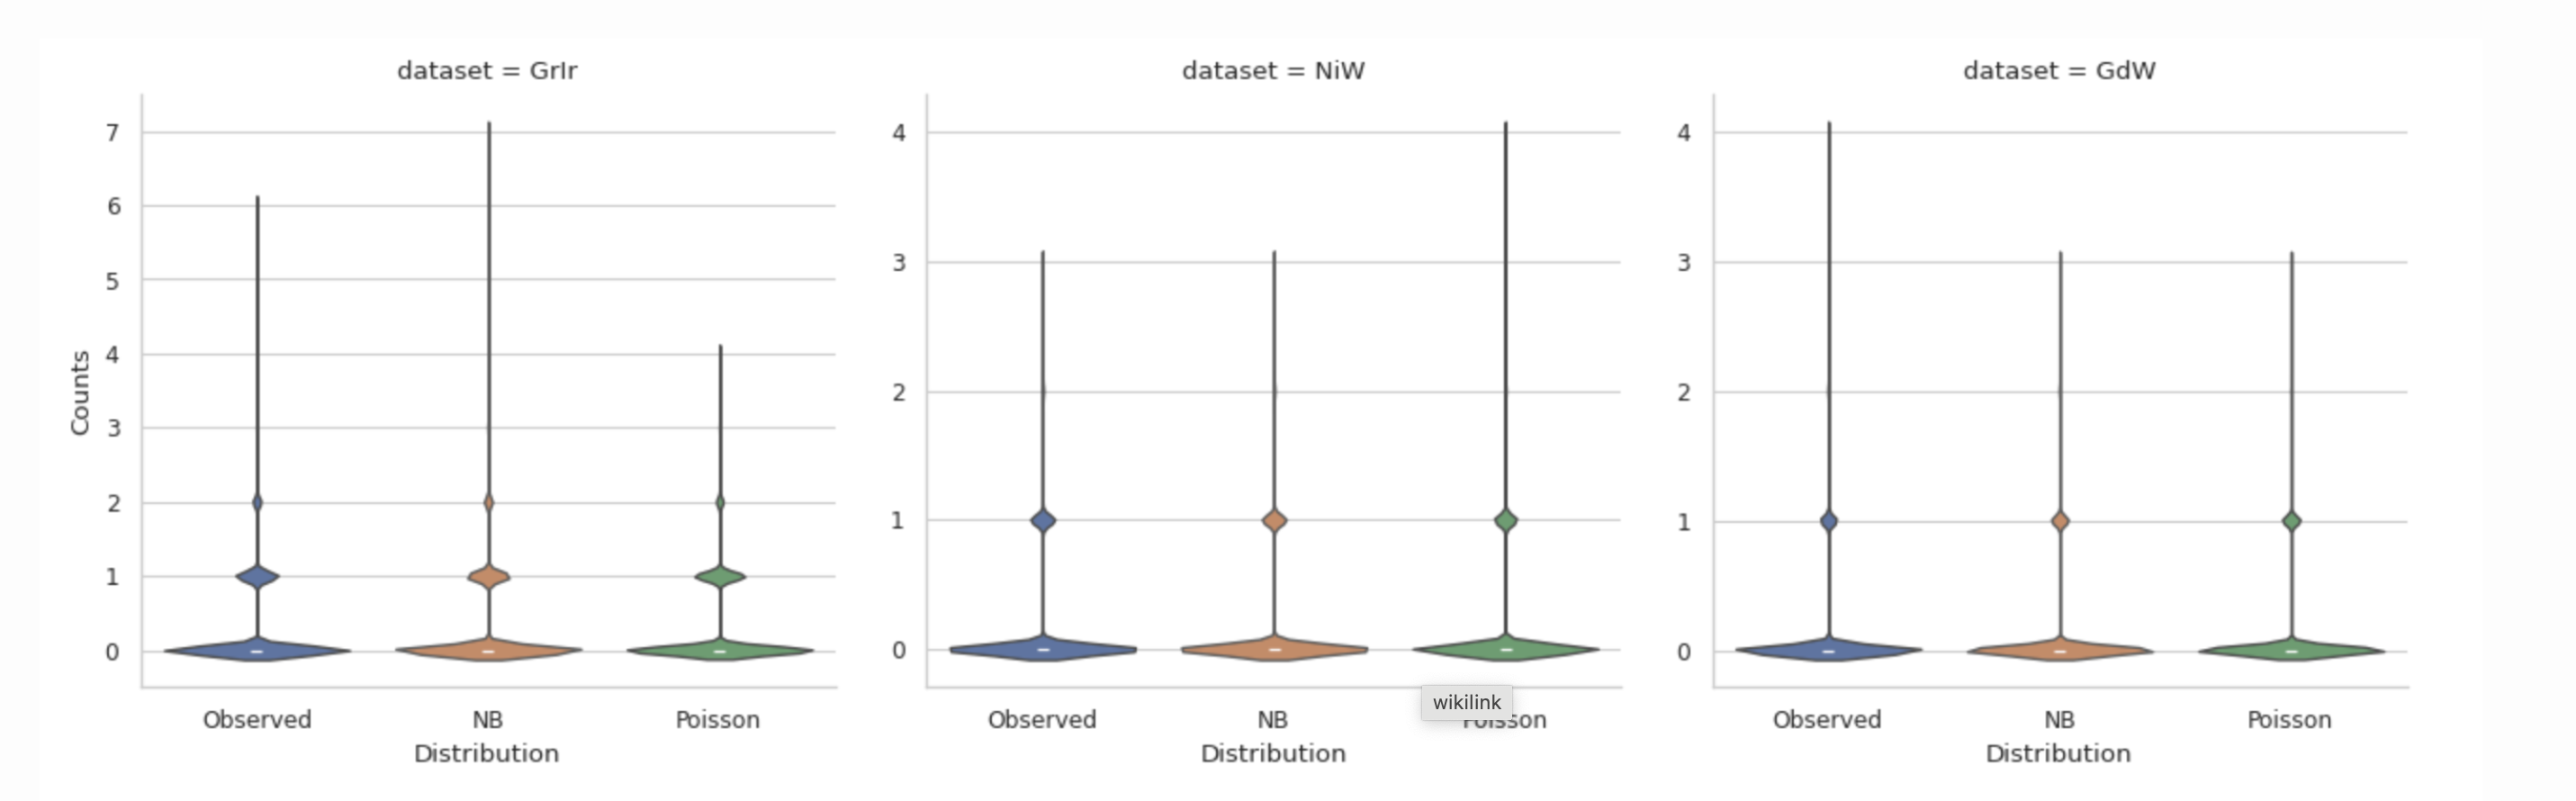
\includegraphics[width=1\linewidth]{images/violin_plots_per_pulse.png}
%     \caption{Enter Caption}
% \end{figure}

% \begin{figure}[htbp]
%     \centering
%     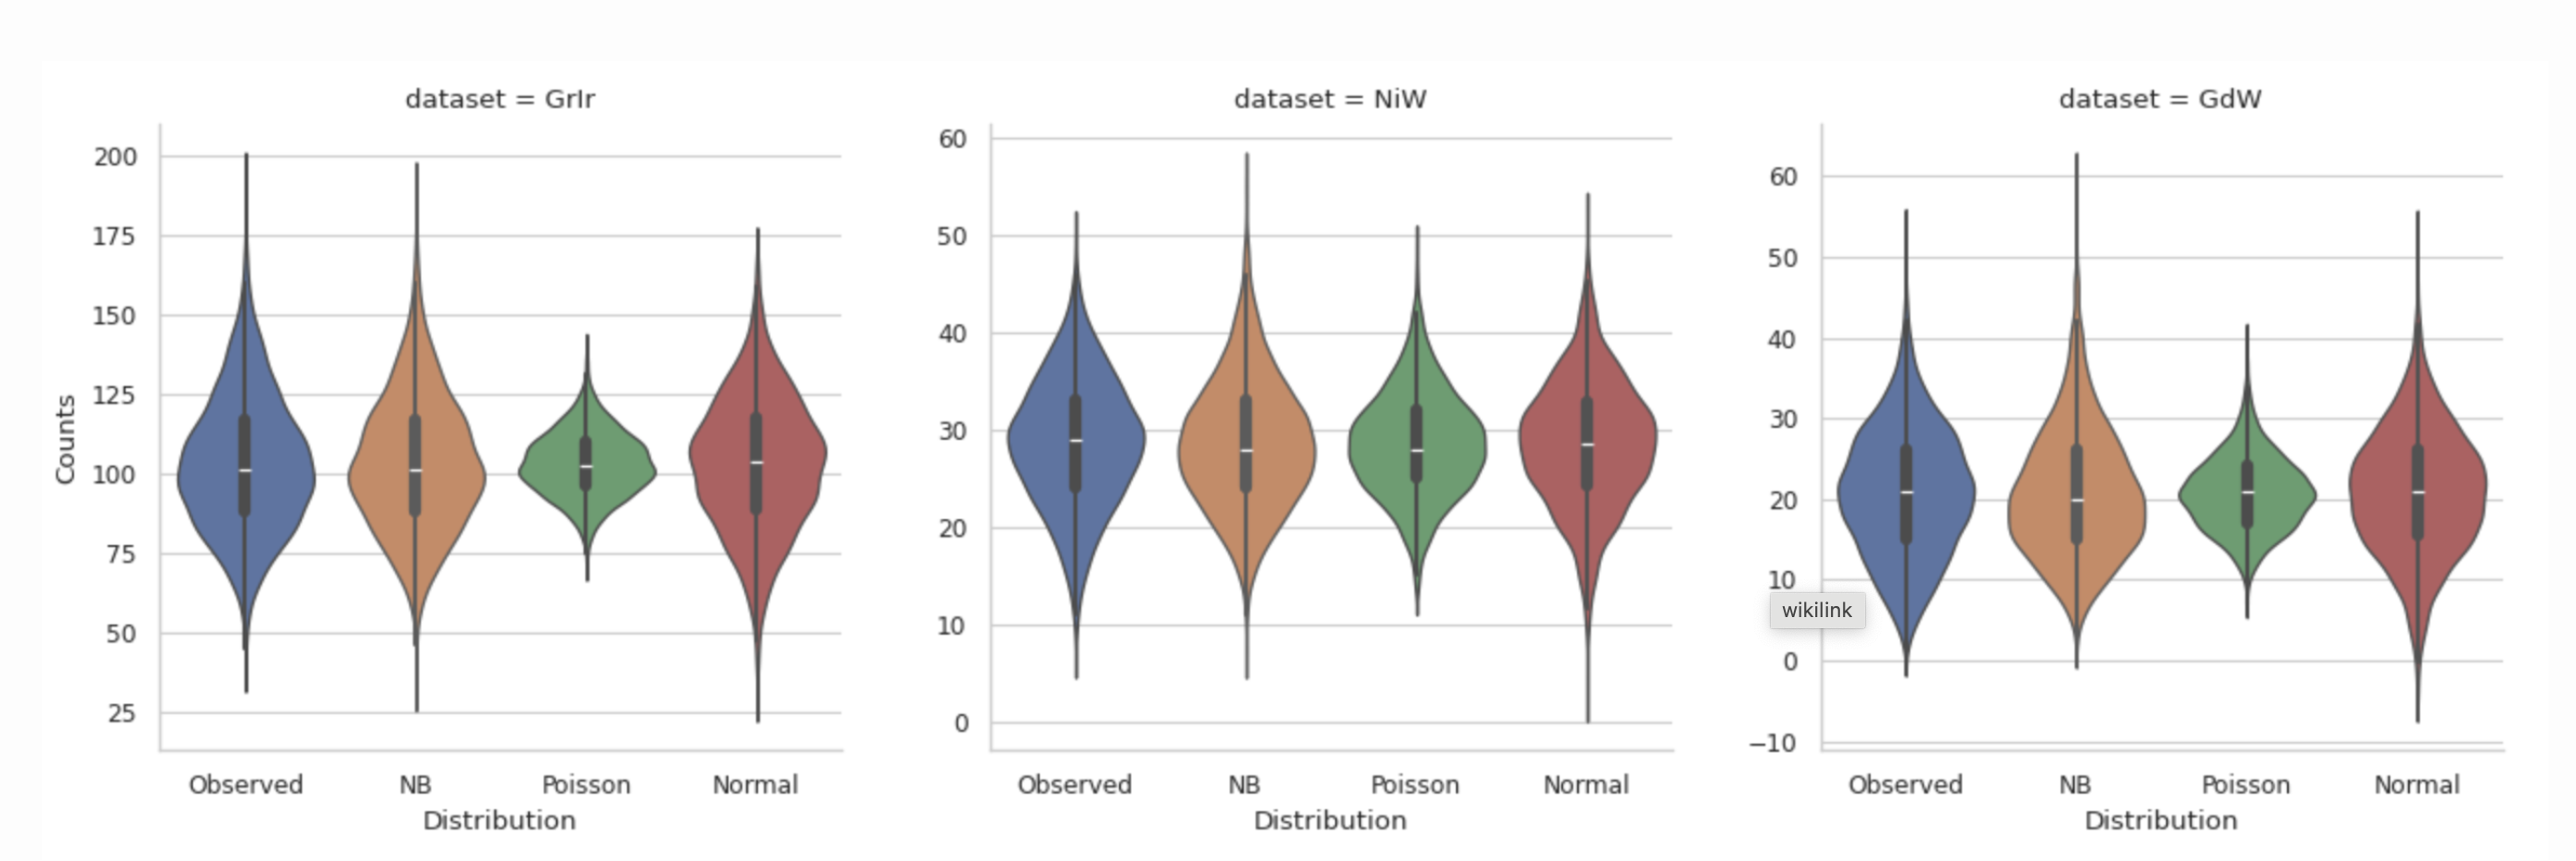
\includegraphics[width=1\linewidth]{images/violinplots_per_train.png}
%     \caption{ss}
%     \label{s}   
% \end{figure}

% \subsection{Analysis of Photoelectron Counting Statistics}